\documentclass[a4paper, 12pt]{article}
\usepackage{xeCJK}
    \setCJKmainfont[AutoFakeBold=1,AutoFakeSlant=.4]{標楷體}
    \XeTeXlinebreaklocale "zh"
    \XeTeXlinebreakskip = 0pt plus 1pt
\usepackage{fontspec}
    \setmainfont{Times New Roman}
\usepackage{setspace}
    \onehalfspace
    \setlength{\parskip}{1ex plus 0.5ex minus 0.2ex}
\usepackage{mathtools}
\usepackage{graphicx}
\usepackage{enumitem}
\usepackage{xcolor}
\graphicspath{{figures/}}
\parindent=0pt
\def\Large{\fontsize{16}{24}\selectfont}
\def\large{\fontsize{14}{20}\selectfont}
\makeatletter
\renewcommand\section{\@startsection {section}{1}{\z@}%
                                   {-3.5ex \@plus -1ex \@minus -.2ex}%
                                   {2.3ex \@plus.2ex}%
                                   {\centering\normalfont\Large\bfseries}}
\renewcommand\subsection{\@startsection {subsection}{1}{\z@}%
                                   {-3.5ex \@plus -1ex \@minus -.2ex}%
                                   {2.3ex \@plus.2ex}%
                                   {\centering\normalfont\large\bfseries}}
\makeatother
\begin{document}

\section*{資料來源}
\subsection*{空氣品質監測資料}
自2017年1月1日至2017年12月31日的高雄地區空氣品質觀測資料,取自於行政院環境保護署空氣品質監測網(https://taqm.epa.gov.tw/taqm/tw/YearlyDataDownload.aspx),當中包含每日每小時的各項監測濃度,我們取用其中的PM2.5、PM10、NO$_\textrm{2}$、NO、SO$_\textrm{2}$、CO與O$_\textrm{3}$,並計算每日的平均作為當日監測資料。
\subsection*{蕁麻疹就診人數資料}
資料來自高雄榮民總醫院(皮膚科),為2017年1月1日至2017年12月31日診斷 ICD-9 代碼為995.3(過敏)每日就診人數資料,此篇為過敏的結果。

\section*{univariate gam}
Generalized additive Poisson model
$$
\ln (patient)=Intercept+\beta \times Air+s(temperature)+
$$
$$
s(humidity)+s(time)+s(rain)+s(windspeed)
$$
s= a cyclic cubic regression splines\\
下列依不同的空汙指標分別做單變數 Generalized additive Poisson model,並以時間趨勢、當天的溫度、濕度、雨量與風速作為共變量做平滑函數的擬合,下列各空汙列出了不同的滯後天數(row,當天~前七天
)與不同的移動平均天數(colum,當天平均~七天平均)的模型結果(p-value與空汙估計係數)
\subsection*{CO}
\begin{table}[h]
\centering
\caption{linear term p-value with lag and moving average data}
\begin{tabular}{rrrrrrrr}
  \hline
 & p.pv & mv2 & mv3 & mv4 & mv5 & mv6 & mv7 \\
  \hline
1 & 0.593 & 0.790 & 0.824 & 0.403 & 0.765 & 0.826 & 0.807 \\
  2 & 0.309 & 0.262 & 0.378 & 0.558 & 0.964 & 0.823 & 0.621 \\
  3 & 0.240 & 0.826 & 0.469 & 0.602 & 0.860 & 0.755 & 0.879 \\
  4 & 0.112 & 0.997 & 0.563 & 0.453 & 0.508 & 0.685 & 0.956 \\
  5 & 0.669 & 0.601 & 0.742 & 0.798 & 0.563 & 0.656 & 0.846 \\
  6 & 0.372 & 0.998 & 0.466 & 0.964 & 0.697 & 0.473 & 0.469 \\
  7 & 0.225 & 0.884 & 0.883 & 0.505 & 0.952 & 0.750 & 0.606 \\
  8 & 0.999 & 0.692 & 0.651 & 0.786 & 0.841 & 0.721 & 0.984 \\
   \hline
\end{tabular}
\\row:lag days,col:moving average for the n days
\end{table}
\begin{table}[h]
\centering
\caption{Parametric coefficients with lag and moving average data}
\begin{tabular}{rrrrrrrr}
  \hline
 & beta & mv2 & mv3 & mv4 & mv5 & mv6 & mv7 \\
  \hline
1 & 0.214 & 0.129 & -0.121 & -0.503 & -0.198 & 0.160 & 0.193 \\
  2 & 0.418 & 0.551 & 0.480 & 0.349 & 0.029 & 0.162 & 0.387 \\
  3 & -0.493 & 0.108 & 0.389 & 0.306 & 0.114 & -0.224 & -0.119 \\
  4 & 0.647 & 0.002 & 0.316 & 0.447 & 0.434 & 0.293 & 0.043 \\
  5 & -0.182 & 0.261 & -0.182 & 0.152 & 0.377 & 0.321 & 0.152 \\
  6 & -0.378 & -0.001 & 0.394 & -0.027 & 0.256 & 0.520 & 0.572 \\
  7 & 0.493 & -0.073 & 0.081 & 0.399 & -0.040 & 0.231 & 0.406 \\
  8 & -0.000 & 0.197 & -0.249 & -0.162 & 0.131 & -0.258 & -0.015 \\
   \hline
\end{tabular}
\end{table}


\clearpage
\subsection*{SO2}
\begin{table}[h]
\centering
\caption{linear term p-value with lag and moving average data}
\begin{tabular}{rrrrrrrr}
  \hline
 & p.pv & mv2 & mv3 & mv4 & mv5 & mv6 & mv7 \\
  \hline
1 & 0.021 & 0.364 & 0.967 & 0.331 & 1.000 & 0.866 & 0.812 \\
  2 & 0.572 & 0.620 & 0.109 & 0.296 & 0.891 & 0.506 & 0.729 \\
  3 & 0.580 & 0.517 & 0.986 & 0.152 & 0.416 & 0.862 & 0.411 \\
  4 & 0.664 & 0.701 & 0.800 & 0.521 & 0.431 & 0.682 & 0.900 \\
  5 & \color{red}{0.038} & 0.389 & 0.621 & 0.671 & 0.966 & 0.229 & 0.378 \\
  6 & 0.670 & 0.212 & 0.421 & 0.584 & 0.605 & 0.846 & 0.211 \\
  7 & 0.662 & 0.132 & 0.540 & 0.331 & 0.255 & 0.255 & 0.137 \\
  8 & 0.292 & 0.307 & 0.808 & 0.545 & 0.842 & 0.916 & 0.943 \\
   \hline
\end{tabular}
\\row:lag days,col:moving average for the n days
\end{table}

\begin{table}[h]
\centering
\caption{Parametric coefficients with lag and moving average data}
\begin{tabular}{rrrrrrrr}
  \hline
 & beta & mv2 & mv3 & mv4 & mv5 & mv6 & mv7 \\
  \hline
1 & -0.107 & 0.051 & 0.003 & -0.070 & 0.000 & -0.014 & -0.020 \\
  2 & 0.026 & -0.028 & 0.104 & 0.074 & 0.010 & 0.054 & 0.029 \\
  3 & 0.025 & 0.037 & 0.001 & 0.102 & 0.062 & 0.014 & 0.070 \\
  4 & -0.020 & -0.022 & -0.016 & -0.046 & 0.061 & 0.033 & -0.011 \\
  5 & \color{red}{0.096} & 0.049 & 0.032 & 0.030 & 0.003 & 0.098 & 0.075 \\
  6 & -0.020 & 0.071 & 0.052 & 0.039 & 0.040 & 0.016 & 0.108 \\
  7 & -0.020 & -0.086 & -0.040 & -0.070 & -0.088 & -0.092 & -0.126 \\
  8 & 0.049 & 0.058 & 0.016 & 0.043 & 0.015 & 0.009 & 0.006 \\
   \hline
\end{tabular}
\end{table}
\begin{figure}[ht!]
       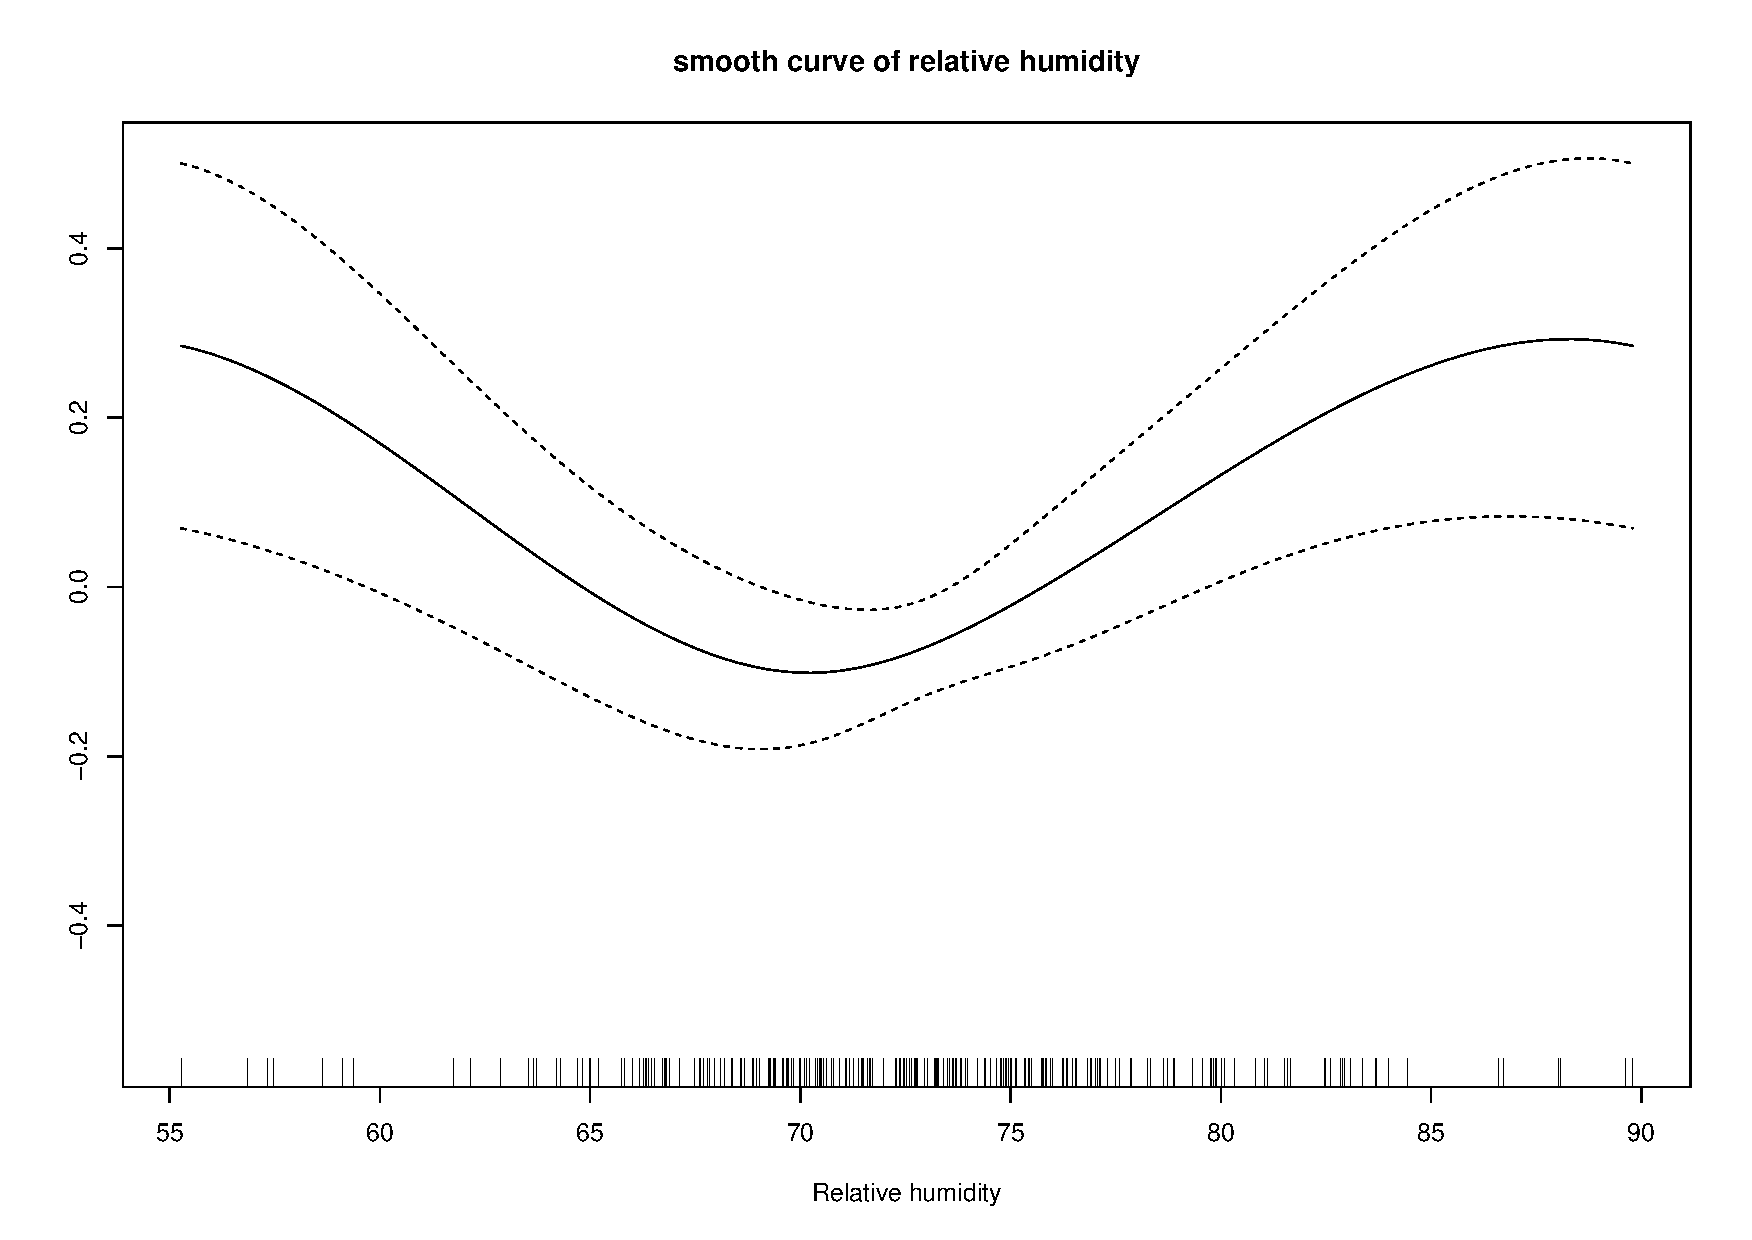
\includegraphics[width=13cm]{RH_SO2.pdf}
       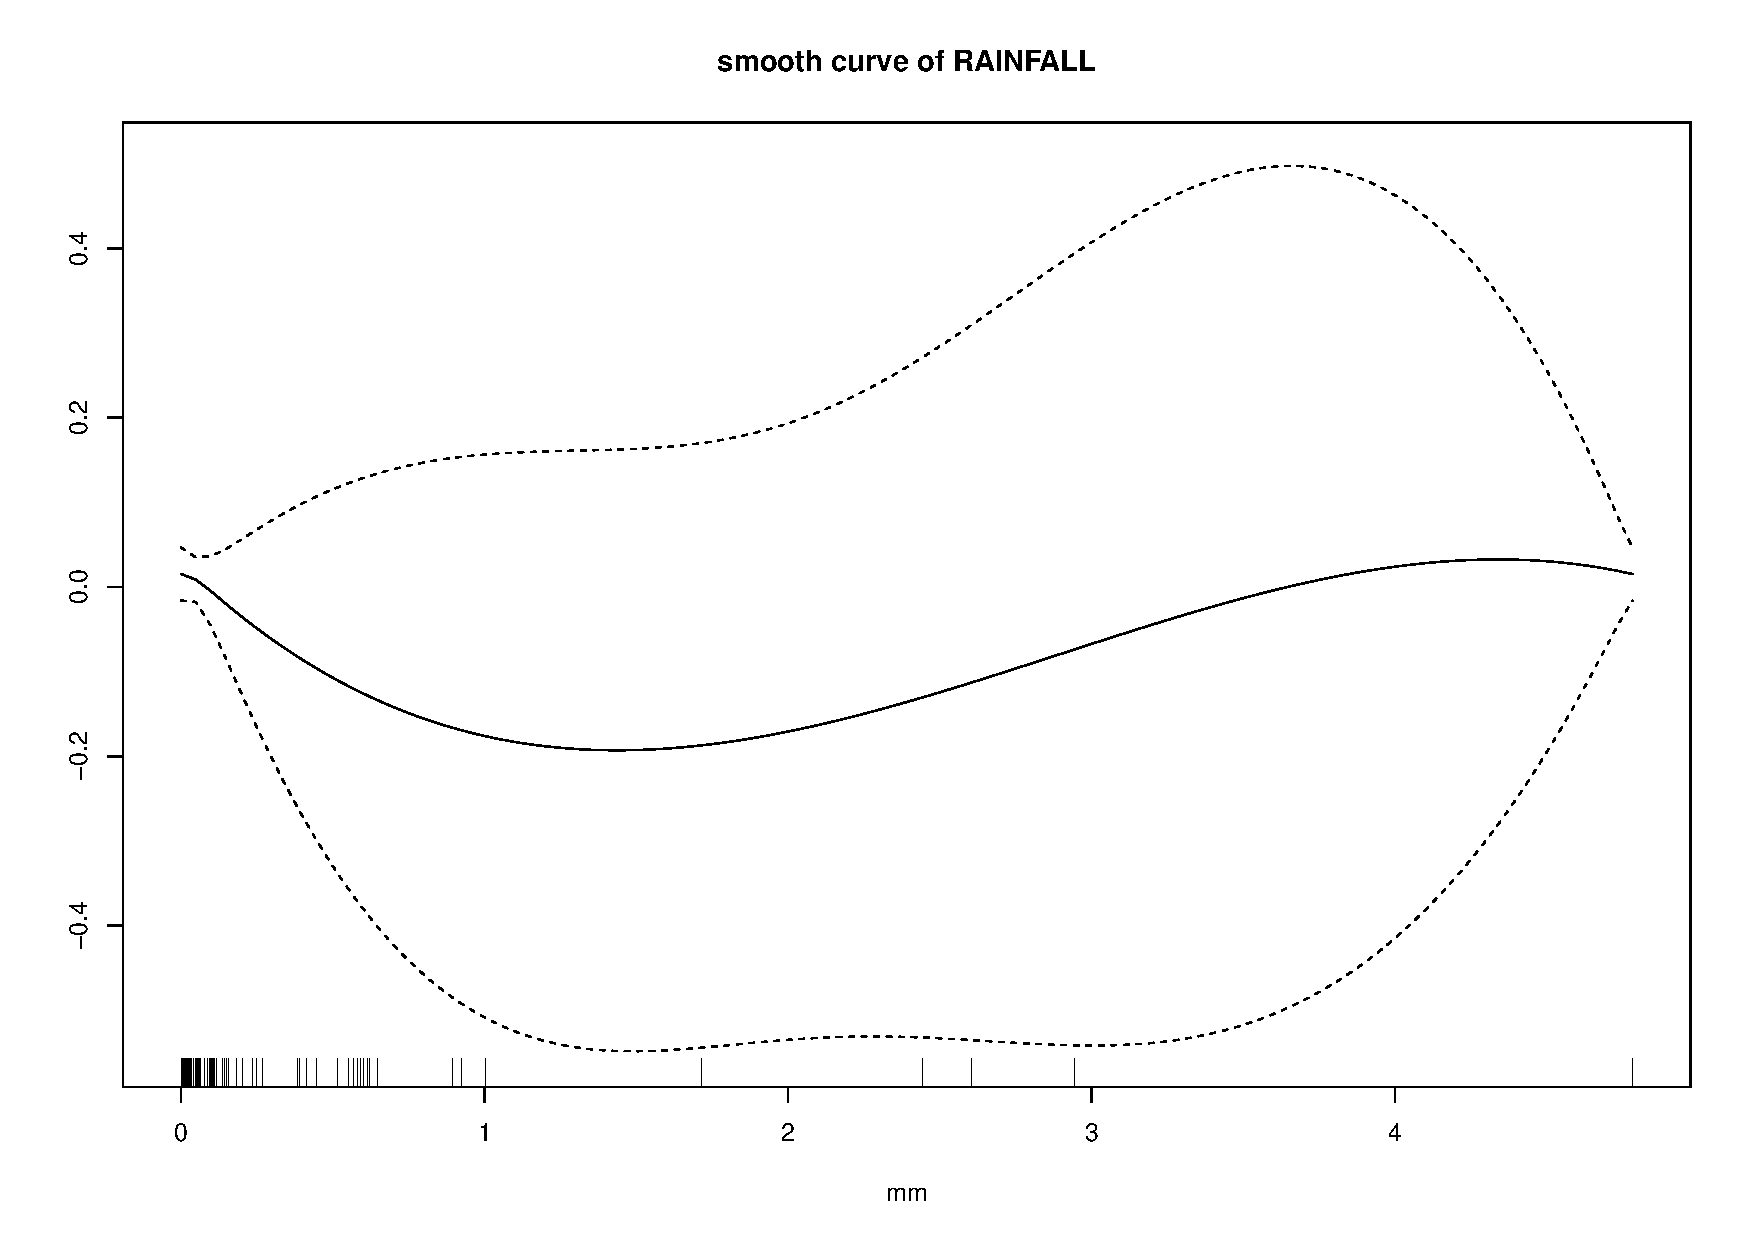
\includegraphics[width=13cm]{RAIN_SO2.pdf}
\end{figure}
\begin{figure}[ht!]
       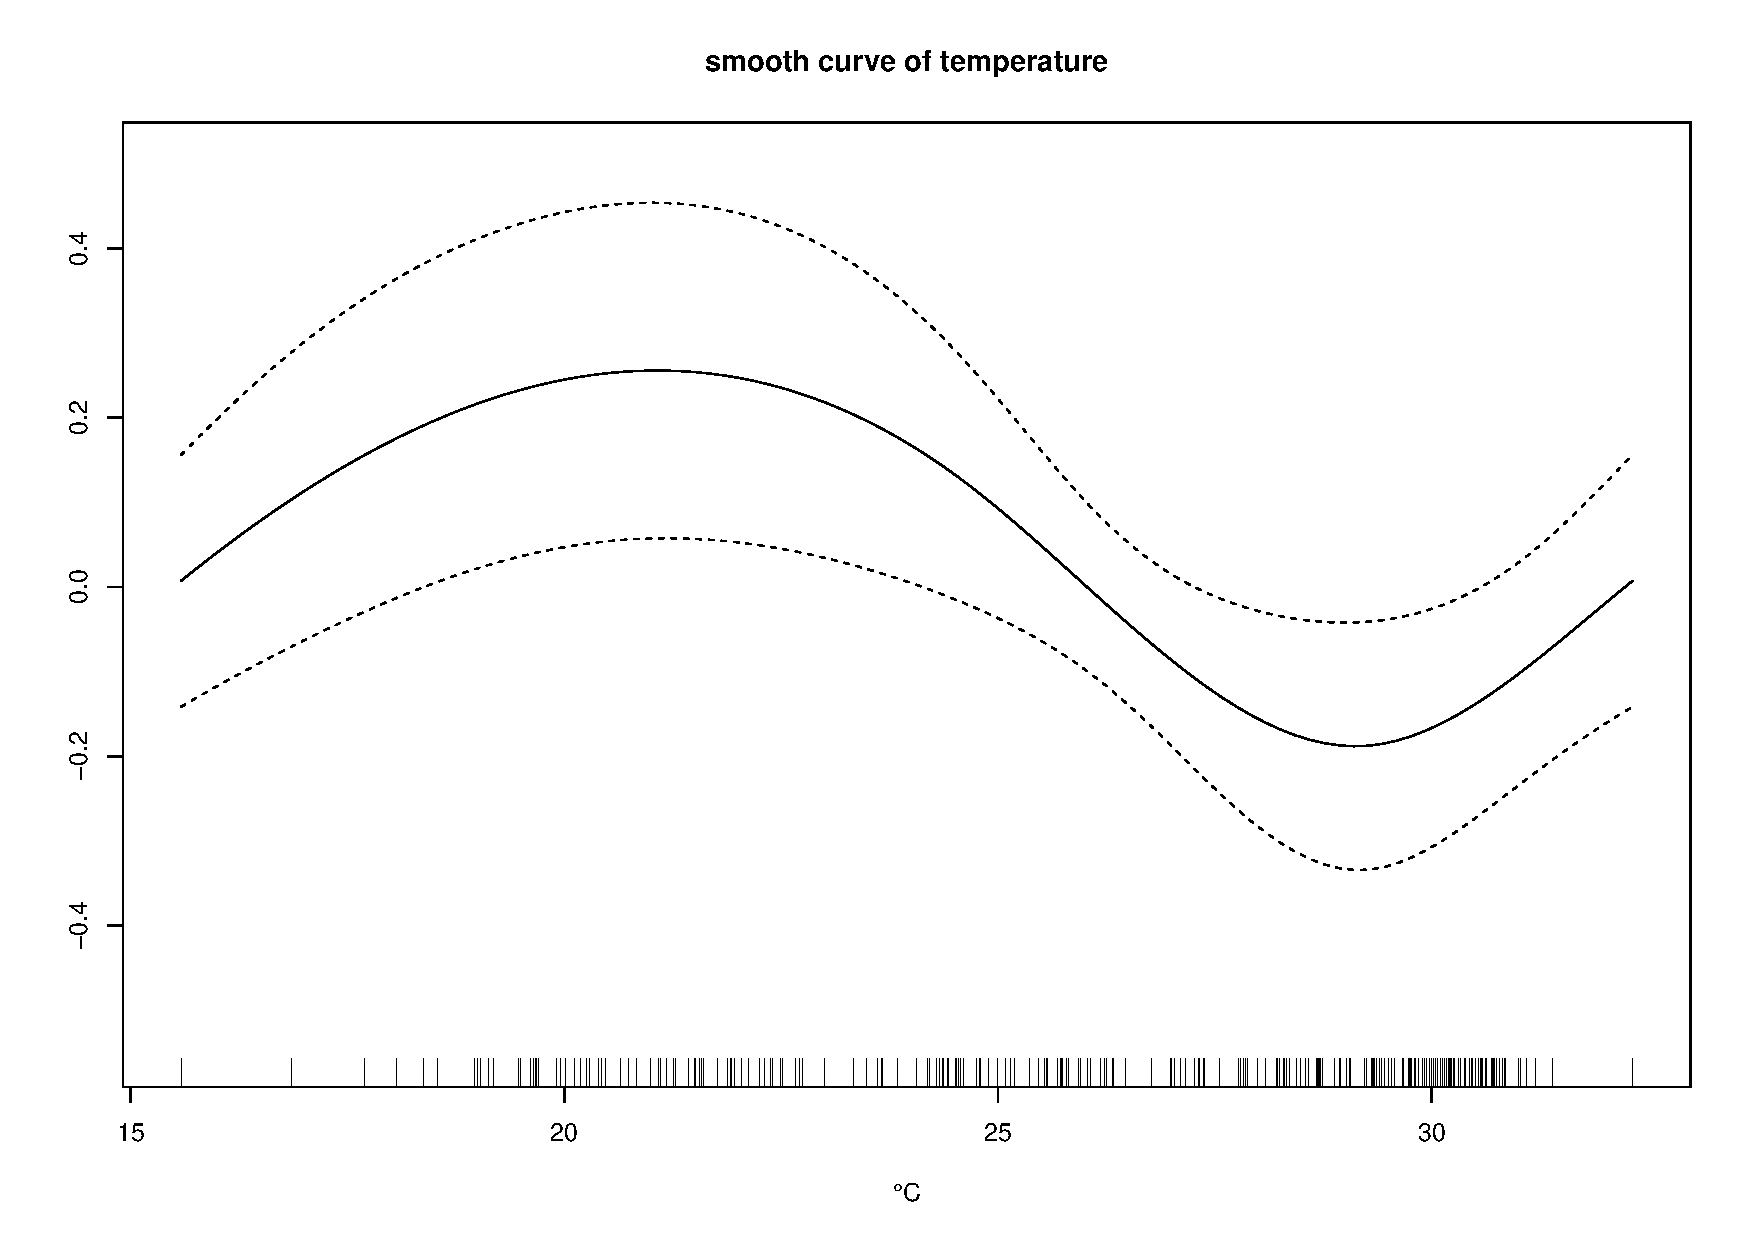
\includegraphics[width=13cm]{TEMP_SO2.pdf}
       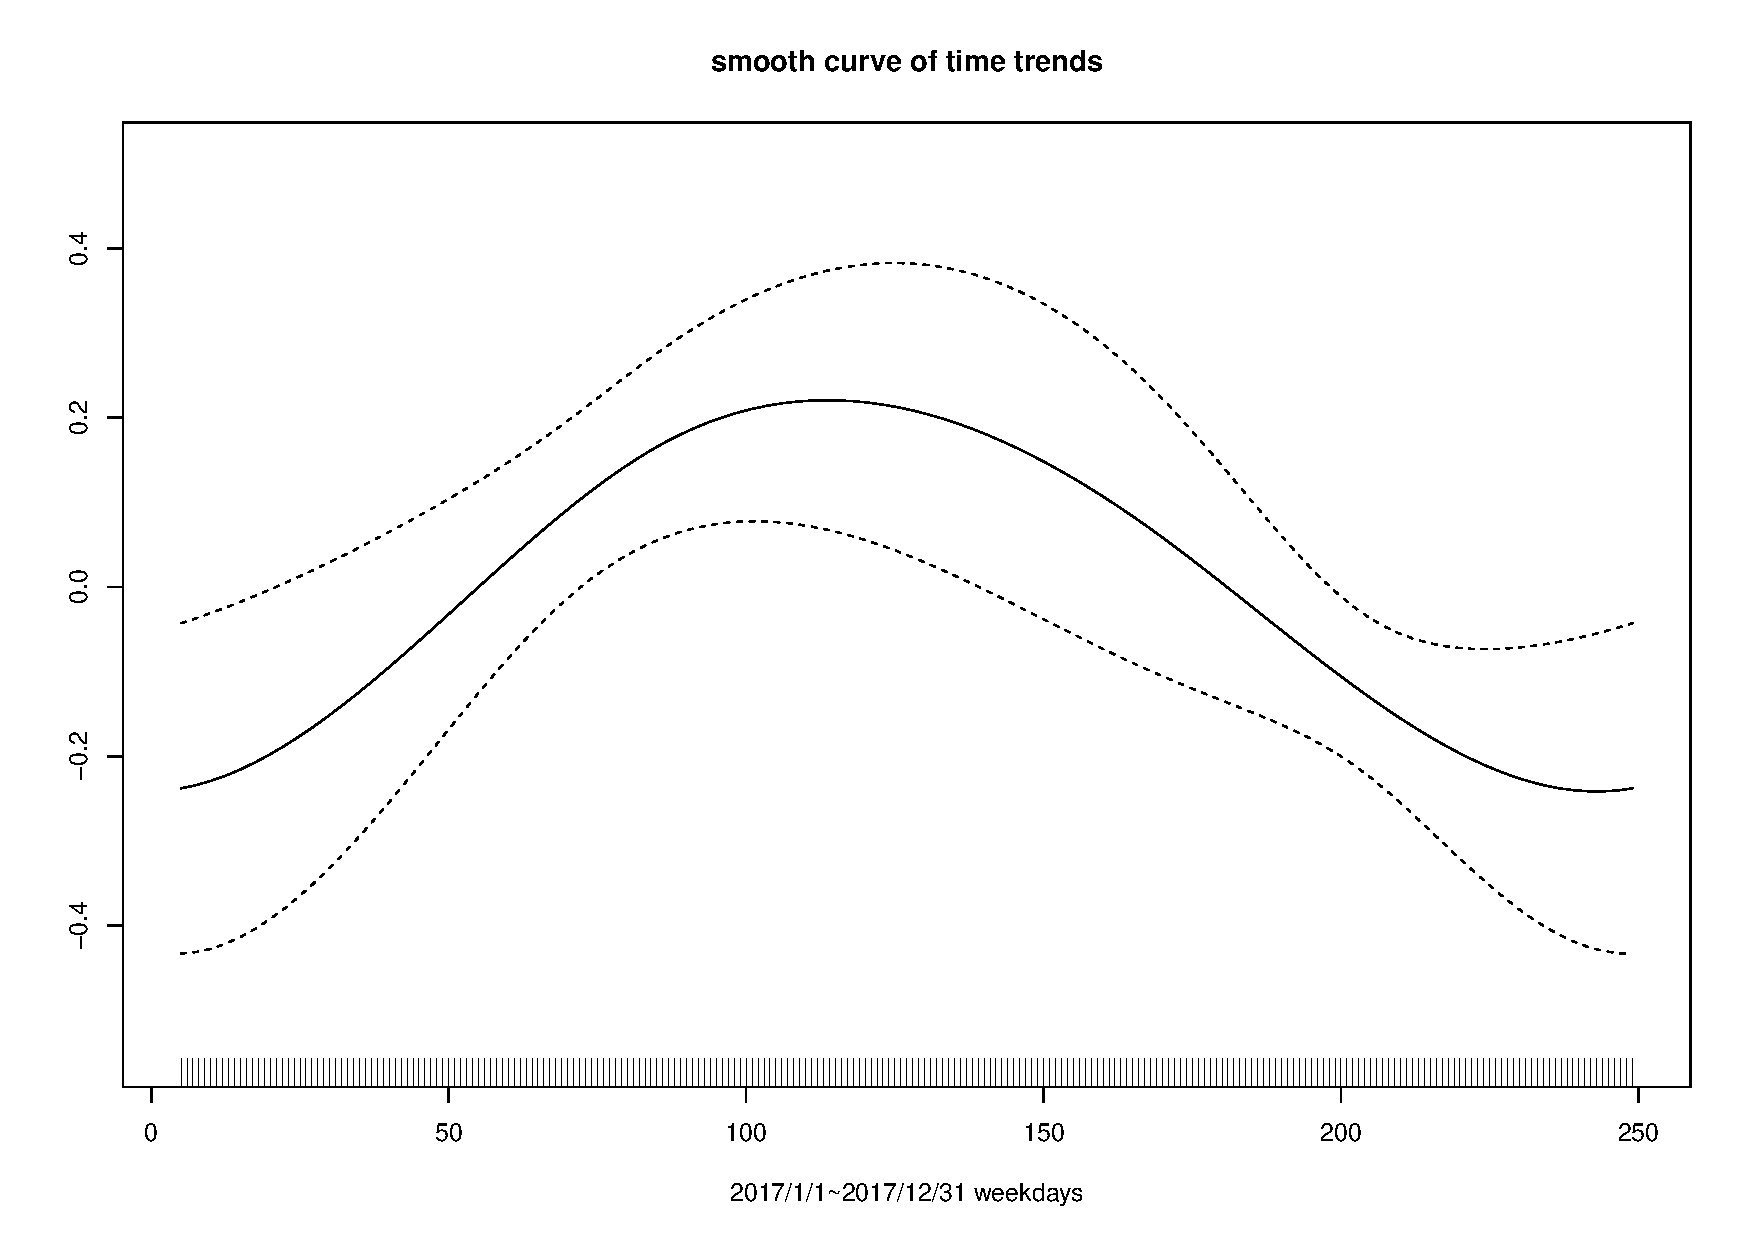
\includegraphics[width=13cm]{TIME_SO2.pdf}
\end{figure}
\begin{figure}[ht!]
       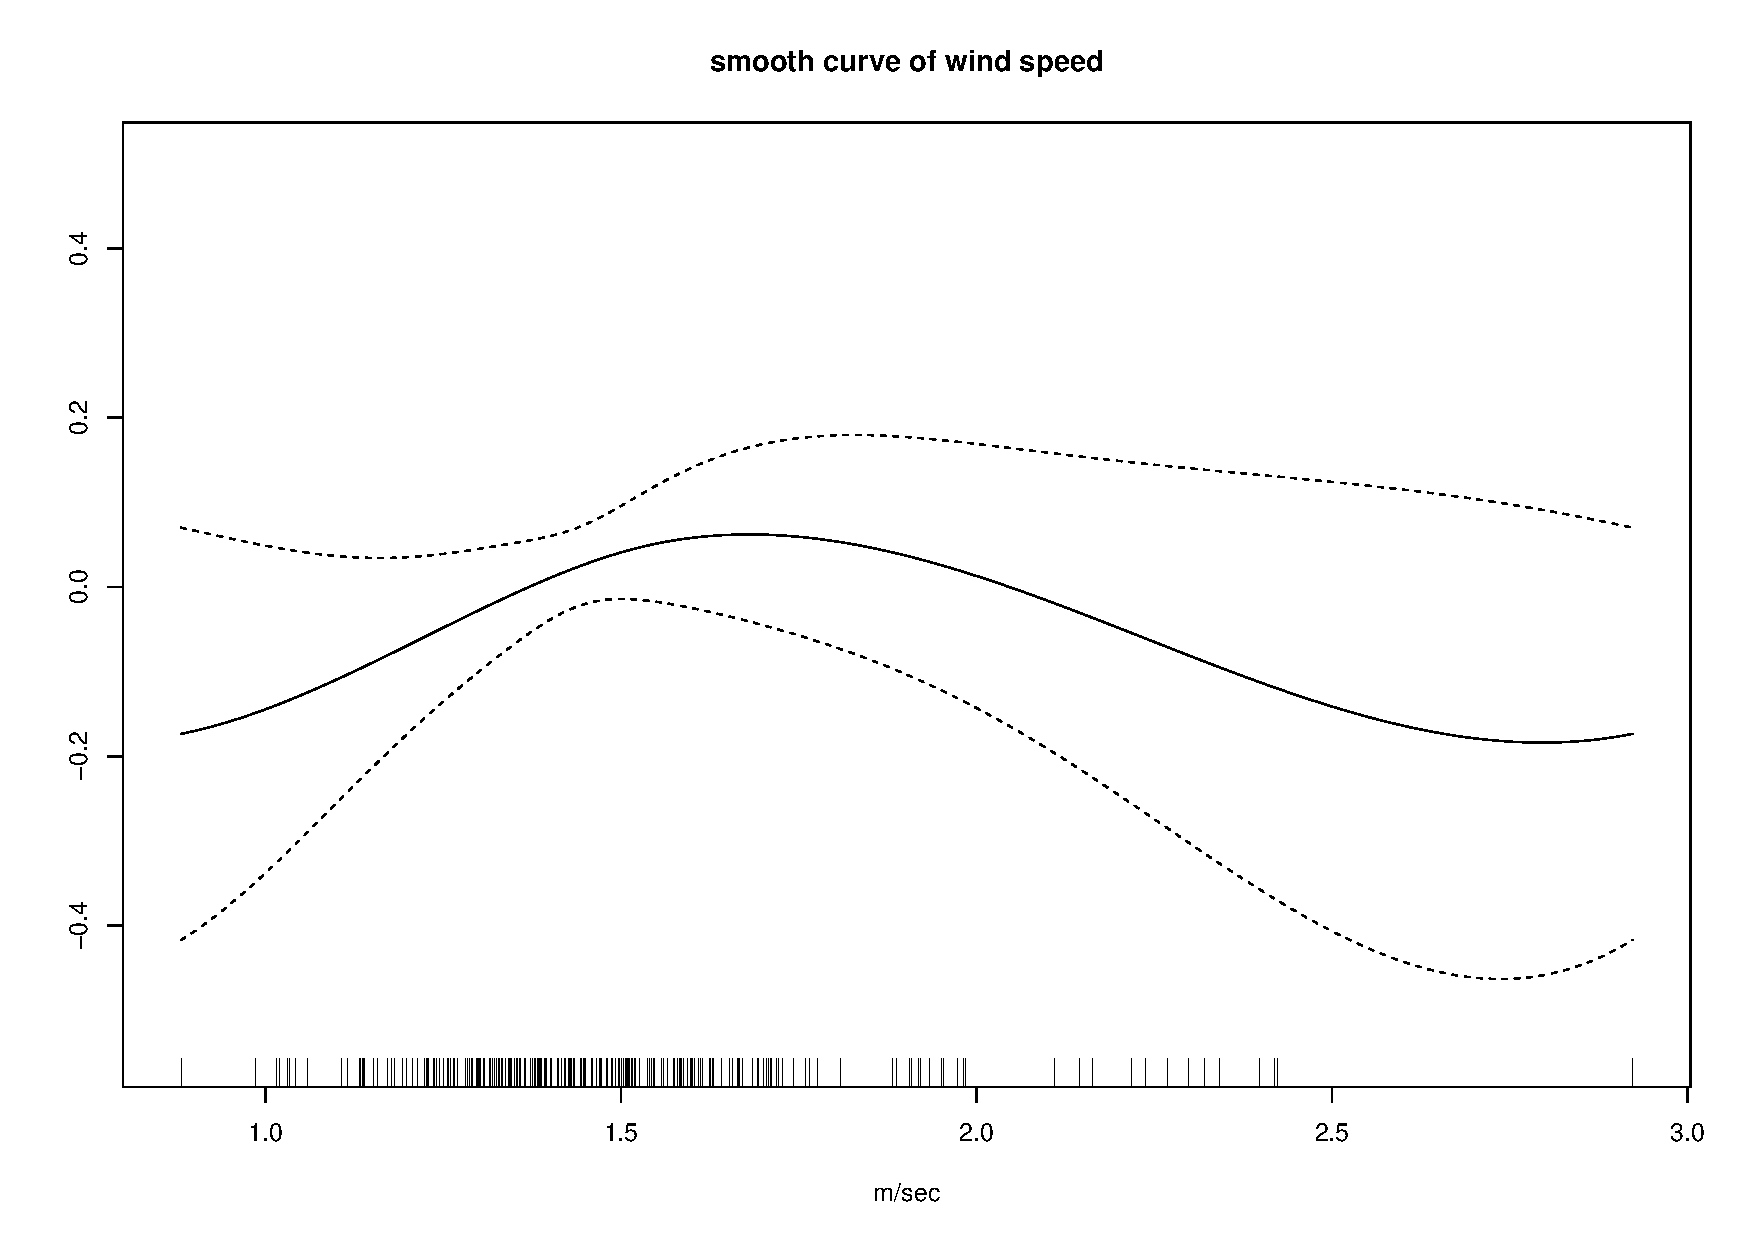
\includegraphics[width=13cm]{WS_SO2.pdf}
\end{figure}

\clearpage
\subsection*{O3}
\begin{table}[h]
\centering
\caption{linear term p-value with lag and moving average data}
\begin{tabular}{rrrrrrrr}
  \hline
 & p.pv & mv2 & mv3 & mv4 & mv5 & mv6 & mv7 \\
  \hline
1 & 0.626 & 0.625 & 0.903 & 0.859 & 0.874 & 0.756 & 0.697 \\
  2 & 0.294 & 0.321 & 0.485 & 0.874 & 0.735 & 0.783 & 0.683 \\
  3 & 0.976 & 0.857 & 0.995 & 0.936 & 0.536 & 0.478 & 0.529 \\
  4 & 0.075 & 0.397 & 0.693 & 0.768 & 0.744 & 0.402 & 0.313 \\
  5 & 0.293 & 0.993 & 0.920 & 0.933 & 0.980 & 0.911 & 0.564 \\
  6 & 0.782 & 0.824 & 0.399 & 0.503 & 0.661 & 0.799 & 0.823 \\
  7 & 0.437 & 0.190 & 0.162 & 0.368 & 0.334 & 0.273 & 0.230 \\
  8 & 0.156 & 0.460 & 0.332 & 0.305 & 0.602 & 0.545 & 0.457 \\
   \hline
\end{tabular}
\\row:lag days,col:moving average for the n days
\end{table}

\begin{table}[h]
\centering
\caption{Parametric coefficients with lag and moving average data}
\begin{tabular}{rrrrrrrr}
  \hline
 & beta & mv2 & mv3 & mv4 & mv5 & mv6 & mv7 \\
  \hline
1 & -0.002 & -0.002 & 0.000 & 0.001 & 0.001 & 0.002 & 0.002 \\
  2 & -0.004 & -0.004 & -0.003 & 0.001 & 0.002 & 0.001 & 0.002 \\
  3 & 0.000 & -0.001 & 0.000 & 0.000 & 0.003 & 0.003 & 0.003 \\
  4 & 0.007 & 0.003 & 0.002 & 0.001 & 0.002 & 0.004 & 0.005 \\
  5 & -0.004 & -0.000 & -0.000 & -0.000 & -0.000 & 0.000 & 0.003 \\
  6 & 0.001 & 0.001 & 0.004 & 0.003 & 0.002 & 0.001 & 0.001 \\
  7 & -0.003 & -0.005 & -0.006 & -0.004 & -0.004 & -0.005 & -0.006 \\
  8 & -0.005 & -0.003 & -0.004 & -0.005 & -0.002 & -0.003 & -0.004 \\
   \hline
\end{tabular}
\end{table}

\clearpage
\subsection*{PM2.5}
\begin{table}[h]
\centering
\caption{linear term p-value with lag and moving average data}
\begin{tabular}{rrrrrrrr}
  \hline
 & p.pv & mv2 & mv3 & mv4 & mv5 & mv6 & mv7 \\
  \hline
1 & 0.290 & 0.149 & 0.630 & 0.585 & 0.627 & 0.367 & 0.115 \\
  2 & \color{red}{0.002} & 0.071 & 0.356 & 0.049 & 0.397 & 0.302 & 0.537 \\
  3 & 0.011 & 0.759 & 0.485 & 0.337 & 0.773 & 0.701 & 0.946 \\
  4 & 0.597 & 0.226 & 0.817 & 0.973 & 0.705 & 0.584 & 0.752 \\
  5 & 0.270 & 0.178 & 0.959 & 0.328 & 0.563 & 0.799 & 0.295 \\
  6 & 0.858 & 0.825 & 0.966 & 0.302 & 0.893 & 0.799 & 0.631 \\
  7 & 0.052 & 0.027 & 0.056 & 0.051 & 0.297 & 0.109 & 0.194 \\
  8 & 0.794 & 0.387 & 0.199 & 0.188 & 0.153 & 0.472 & 0.161 \\
   \hline
\end{tabular}
\\row:lag days,col:moving average for the n days
\end{table}

\begin{table}[h]
\centering
\caption{Parametric coefficients with lag and moving average data}
\begin{tabular}{rrrrrrrr}
  \hline
 & beta & mv2 & mv3 & mv4 & mv5 & mv6 & mv7 \\
  \hline
1 & 0.004 & 0.008 & -0.003 & 0.004 & 0.003 & 0.007 & 0.013 \\
  2 & \color{red}{-0.013} & -0.010 & -0.006 & -0.013 & -0.006 & -0.008 & -0.005 \\
  3 & 0.011 & 0.002 & 0.004 & 0.006 & -0.002 & 0.003 & -0.000 \\
  4 & -0.002 & 0.006 & -0.001 & 0.000 & 0.003 & -0.004 & 0.002 \\
  5 & -0.005 & -0.007 & -0.000 & -0.006 & -0.004 & -0.002 & -0.008 \\
  6 & -0.001 & 0.001 & 0.000 & 0.007 & 0.001 & 0.002 & 0.004 \\
  7 & -0.008 & -0.012 & -0.012 & -0.013 & -0.007 & -0.012 & -0.010 \\
  8 & 0.001 & -0.005 & -0.008 & -0.009 & -0.010 & -0.005 & -0.011 \\
   \hline
\end{tabular}
\end{table}
\clearpage
\subsection*{PM10}
\begin{table}[h]
\centering
\caption{linear term p-value with lag and moving average data}
\begin{tabular}{rrrrrrrr}
  \hline
 & p.pv & mv2 & mv3 & mv4 & mv5 & mv6 & mv7 \\
  \hline
1 & 0.005 & 0.095 & 0.500 & 0.785 & 0.922 & 0.844 & 0.166 \\
  2 & 0.186 & 0.354 & 0.455 & 0.389 & 0.777 & 0.790 & 0.976 \\
  3 & 0.089 & 0.761 & 0.079 & 0.131 & 0.978 & 0.652 & 0.731 \\
  4 & 0.109 & 0.948 & 0.536 & 0.438 & 0.471 & 0.619 & 0.945 \\
  5 & 0.061 & 0.944 & 0.520 & 0.881 & 0.166 & 0.190 & 0.901 \\
  6 & 0.345 & 0.215 & 0.840 & 0.410 & 0.753 & 0.212 & 0.270 \\
  7 & \color{red}{0.000} & 0.001 & 0.131 & 0.031 & 0.138 & 0.074 & 0.410 \\
  8 & 0.895 & 0.028 & 0.007 & 0.180 & 0.070 & 0.231 & 0.117 \\
   \hline
\end{tabular}
\\row:lag days,col:moving average for the n days
\end{table}

\begin{table}[h]
\centering
\caption{Parametric coefficients with lag and moving average data}
\begin{tabular}{rrrrrrrr}
  \hline
 & beta & mv2 & mv3 & mv4 & mv5 & mv6 & mv7 \\
  \hline
1 & 0.005 & 0.004 & -0.002 & -0.001 & -0.000 & 0.001 & 0.006 \\
  2 & -0.003 & 0.002 & 0.002 & -0.003 & -0.001 & -0.001 & -0.000 \\
  3 & 0.003 & 0.001 & 0.005 & 0.005 & -0.000 & 0.002 & 0.001 \\
  4 & -0.003 & -0.000 & -0.002 & 0.003 & 0.003 & -0.002 & 0.000 \\
  5 & 0.004 & -0.000 & 0.002 & 0.000 & 0.005 & 0.005 & 0.000 \\
  6 & -0.002 & 0.003 & 0.001 & 0.003 & 0.001 & 0.005 & 0.005 \\
  7 & \color{red}{-0.008} & -0.009 & -0.005 & -0.007 & -0.005 & -0.007 & -0.003 \\
  8 & 0.000 & -0.006 & -0.008 & -0.004 & -0.007 & -0.005 & -0.006 \\
   \hline
\end{tabular}
\end{table}
\clearpage
\subsection*{NO}
\begin{table}[h]
\centering
\caption{linear term p-value with lag and moving average data}
\begin{tabular}{rrrrrrrr}
  \hline
 & p.pv & mv2 & mv3 & mv4 & mv5 & mv6 & mv7 \\
  \hline
1 & 0.525 & 0.411 & 0.854 & 0.370 & 0.561 & 0.721 & 0.547 \\
  2 & 0.099 & 0.823 & 0.889 & 0.604 & 0.314 & 0.491 & 0.561 \\
  3 & 0.949 & 0.336 & 0.751 & 0.944 & 0.463 & 0.246 & 0.430 \\
  4 & 0.522 & 0.431 & 0.159 & 0.403 & 0.501 & 0.204 & 0.080 \\
  5 & 0.270 & 0.471 & 0.686 & 0.748 & 0.965 & 0.921 & 0.531 \\
  6 & 0.611 & 0.682 & 0.879 & 0.810 & 0.422 & 0.752 & 0.909 \\
  7 & 0.255 & 0.417 & 0.174 & 0.205 & 0.304 & 0.567 & 0.365 \\
  8 & 0.611 & 0.520 & 0.604 & 0.276 & 0.333 & 0.390 & 0.607 \\
   \hline
\end{tabular}
\\row:lag days,col:moving average for the n days
\end{table}

\begin{table}[h]
\centering
\caption{Parametric coefficients with lag and moving average data}
\begin{tabular}{rrrrrrrr}
  \hline
 & beta & mv2 & mv3 & mv4 & mv5 & mv6 & mv7 \\
  \hline
1 & 0.019 & 0.028 & -0.007 & -0.038 & -0.026 & -0.017 & -0.030 \\
  2 & -0.050 & -0.008 & 0.005 & -0.022 & -0.046 & -0.033 & -0.029 \\
  3 & 0.002 & -0.034 & -0.012 & -0.003 & -0.033 & -0.056 & -0.040 \\
  4 & -0.019 & -0.027 & -0.055 & -0.036 & -0.030 & -0.061 & -0.088 \\
  5 & 0.032 & 0.025 & 0.016 & -0.014 & -0.002 & -0.005 & -0.032 \\
  6 & -0.015 & 0.014 & 0.006 & -0.010 & -0.036 & -0.015 & -0.006 \\
  7 & 0.034 & 0.028 & 0.052 & 0.053 & 0.046 & 0.028 & 0.046 \\
  8 & 0.015 & 0.022 & 0.020 & 0.046 & 0.043 & 0.041 & 0.026 \\
   \hline
\end{tabular}
\end{table}
\clearpage
\subsection*{NO2}
\begin{table}[h]
\centering
\caption{linear term p-value with lag and moving average data}
\begin{tabular}{rrrrrrrr}
  \hline
 & p.pv & mv2 & mv3 & mv4 & mv5 & mv6 & mv7 \\
  \hline
1 & 0.229 & 0.424 & 0.285 & 0.319 & 0.303 & 0.605 & 0.735 \\
  2 & \color{red}{0.000} & 0.206 & 0.468 & 0.092 & 0.157 & 0.112 & 0.221 \\
  3 & 0.403 & 0.230 & 0.942 & 0.967 & 0.268 & 0.331 & 0.313 \\
  4 & 0.004 & 0.062 & 0.005 & 0.081 & 0.149 & 0.022 & 0.041 \\
  5 & 0.606 & 0.172 & 0.312 & 0.066 & 0.289 & 0.333 & 0.095 \\
  6 & 0.862 & 0.209 & 0.947 & 0.992 & 0.334 & 0.769 & 0.893 \\
  7 & 0.062 & 0.075 & 0.517 & 0.178 & 0.207 & 0.045 & 0.138 \\
  8 & 0.105 & 0.708 & 0.445 & 0.918 & 0.434 & 0.482 & 0.158 \\
   \hline
\end{tabular}
\\row:lag days,col:moving average for the n days
\end{table}

\begin{table}[h]
\centering
\caption{Parametric coefficients with lag and moving average data}
\begin{tabular}{rrrrrrrr}
  \hline
 & beta & mv2 & mv3 & mv4 & mv5 & mv6 & mv7 \\
  \hline
1 & 0.015 & 0.011 & -0.017 & -0.017 & -0.019 & -0.010 & -0.007 \\
  2 & \color{red}{-0.050} & -0.018 & -0.011 & -0.029 & -0.026 & -0.032 & -0.026 \\
  3 & 0.011 & -0.018 & -0.001 & 0.001 & -0.020 & -0.019 & -0.022 \\
  4 & -0.038 & -0.028 & -0.046 & -0.030 & -0.027 & -0.046 & -0.043 \\
  5 & 0.007 & -0.020 & -0.016 & -0.032 & -0.019 & -0.019 & -0.035 \\
  6 & -0.002 & 0.018 & 0.001 & -0.000 & -0.018 & -0.006 & -0.003 \\
  7 & -0.025 & -0.026 & -0.010 & -0.023 & -0.024 & -0.040 & -0.031 \\
  8 & 0.021 & -0.005 & -0.012 & -0.002 & -0.015 & -0.014 & -0.030 \\
   \hline
\end{tabular}
\end{table}


\end{document} 